\chapter{Architecture}
 
\begin{figure}[!h]
\begin{center}
  \fbox{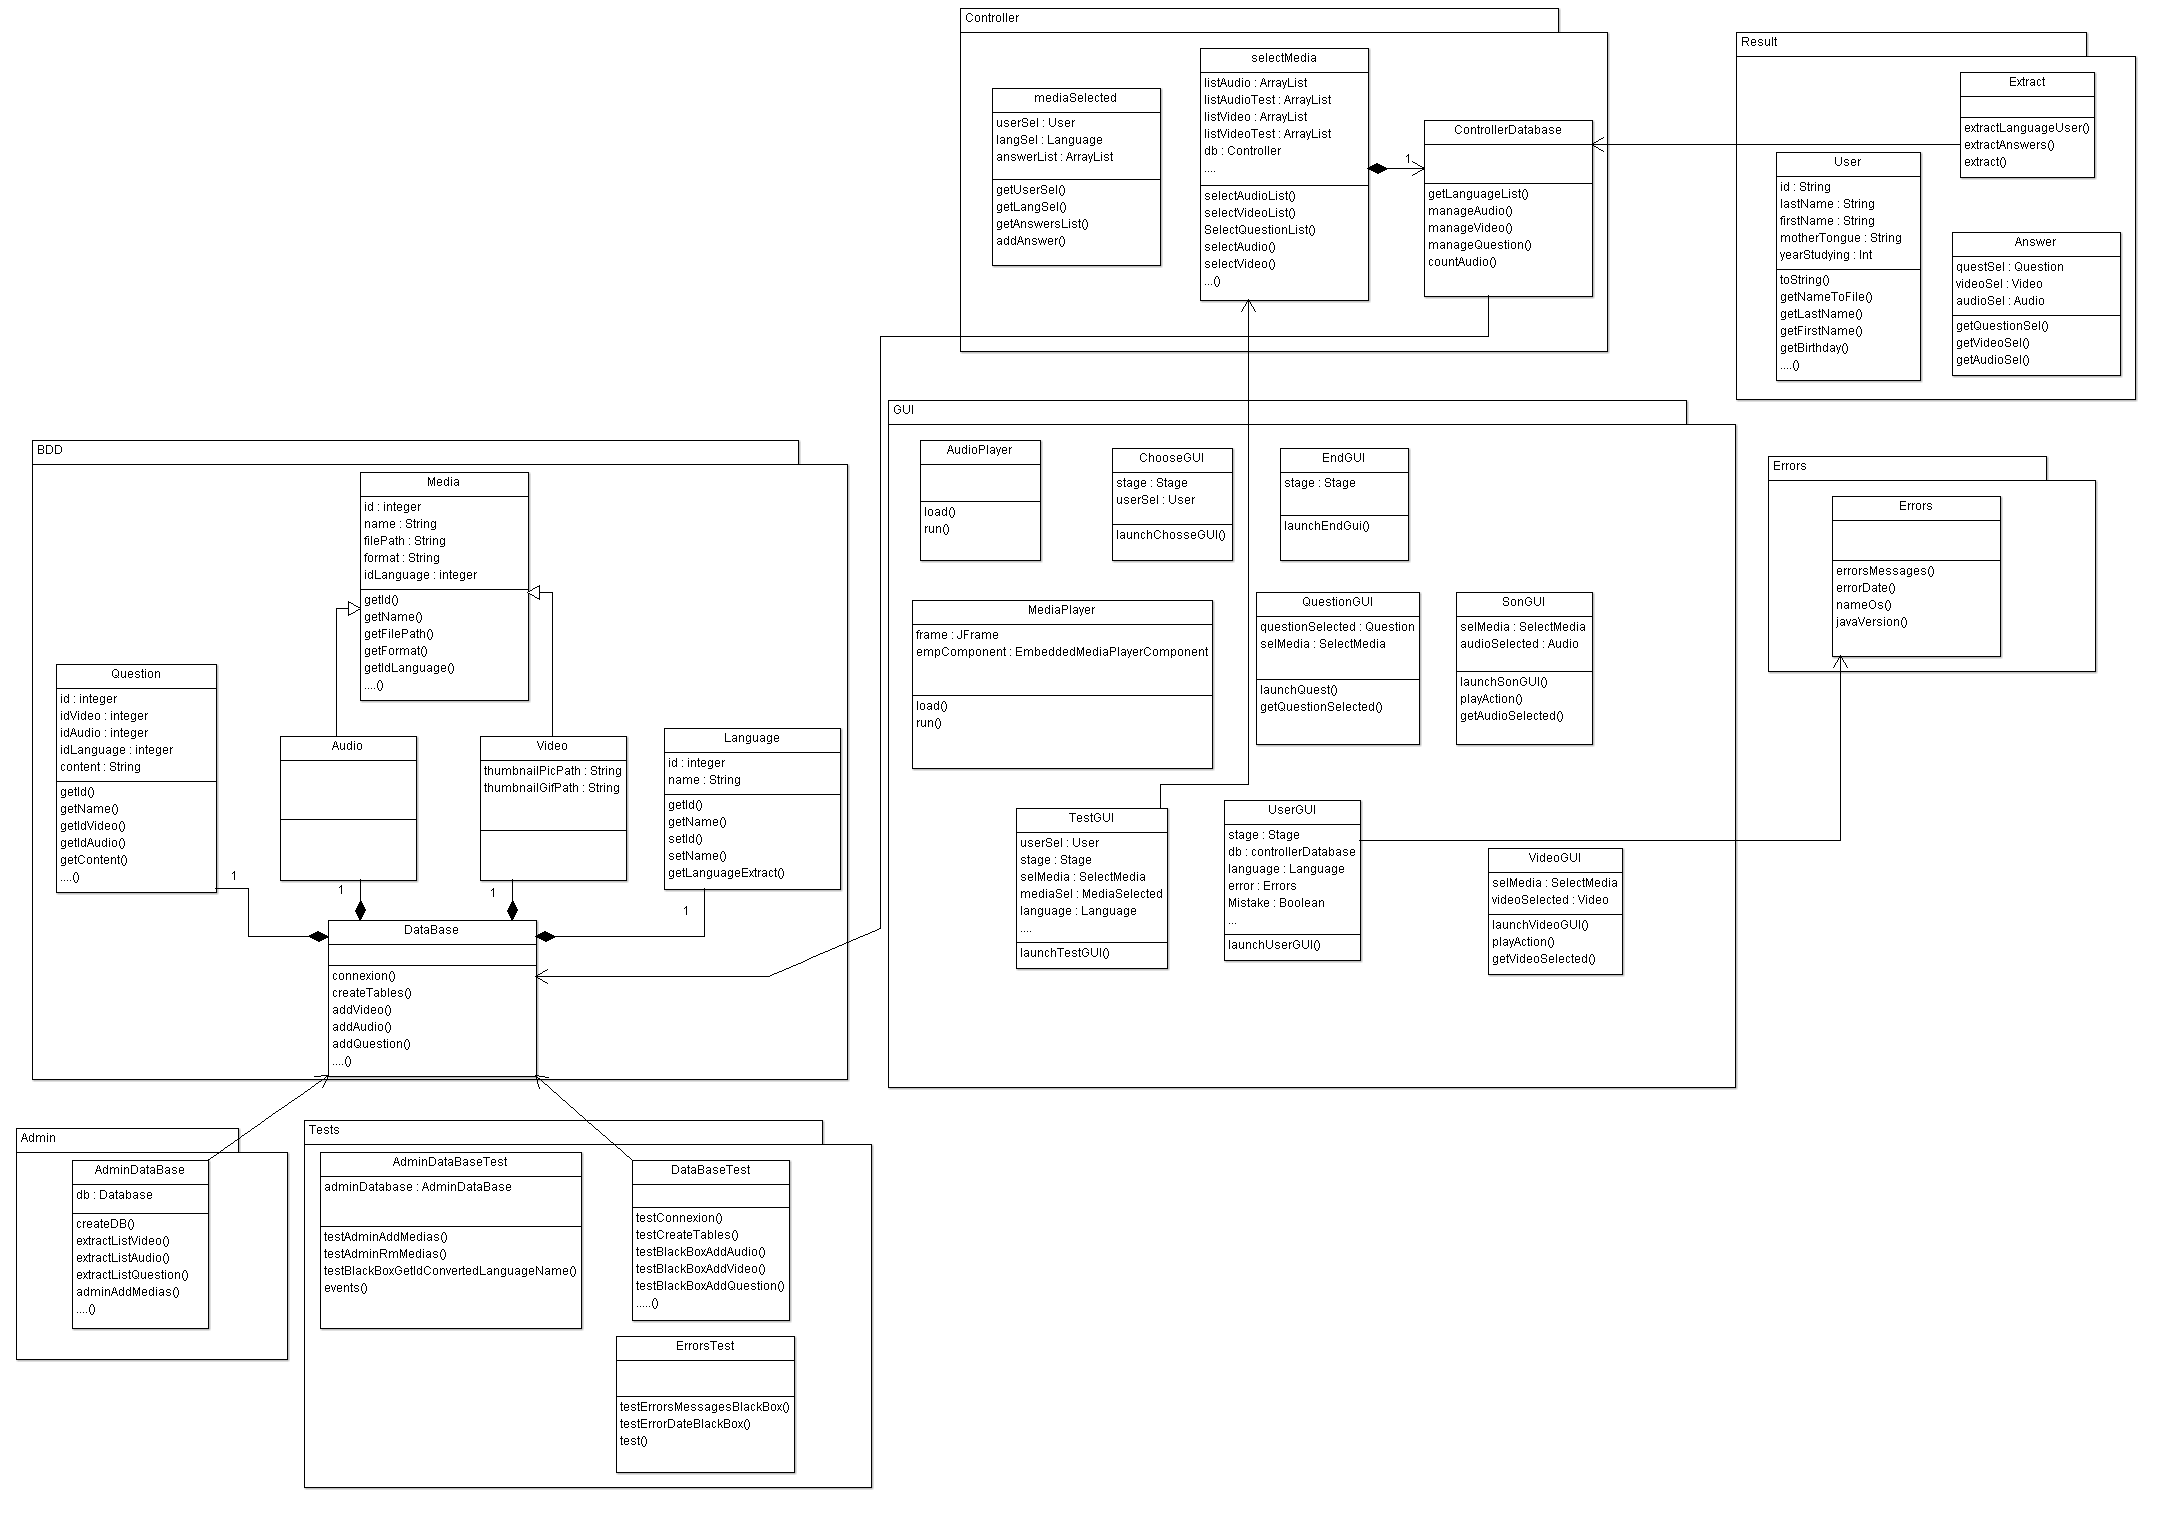
\includegraphics[width=18cm,angle=90]{./architecture/architecture.png}}
  \caption{UML - Architecture}
  \label{diaglog} 
\end{center}
\end{figure}

L'architecture \textbf{M}odele-\textbf{V}ue-\textbf{C}ontroleur (\textbf{MVC}) permettant ``la séparation des éléments principaux d'un système d'intéraction d'une couche présentation''\footnote{Citation du cours magistral de PdP de M.Narbel} nous semblait le pattern le mieux adapté au développement de notre application basée sur les liens base de données/interface graphique. 

De plus, grâce à ce \textit{design pattern}, nous avons pu répartir les rôles de chacun afin de produire un travail efficace.

\section{Explication détaillée des packages}

Notre architecture est structuré en plusieurs packages. Ils ont été créés avec comme but de compartimenter notre architecture en fonction des besoins renseignés précédemment. Chaque package regroupe un certain nombre de classes, chacune possédant une fonction bien précise.

Dans cette section, nous allons décrire le besoin que nous avons voulu satisfaire avec chaque package et le rôle de chacune de leurs classes. Pour suivre la logique MVC, nous allons structurer la description selon ce même pattern.

\subsection{Modèle}


\subsubsection{BDD}

Ce package concerne tout ce qui se rapproche de la base de données. Ainsi, elle possède tous les types d'objets que nous allons insérer et sélectionner :
\begin{itemize}
 \item \textit{Media}
  \subitem \textit{Video}
  \subitem \textit{Audio}
 \item \textit{Language}
 \item \textit{Question}
\end{itemize}


Ces types d'objet intéragissent avec la base de données via la classe \textit{Database}.

Nouvelle langue > simple et rapide.

\paragraph{Classe DataBase}

Cette classe contient toutes les intéractions entre les objets et la base de données (on notera BDD dès à présent). Elle permet de :

\begin{itemize}
 \item se connecter à la BDD (créer et initialiser la BDD le cas échéant)
 \item remplir la BDD
 \item rechercher dans la BDD
 \item supprimer des éléments dans la BDD
 \item consulter la BDD
\end{itemize}


Cette centralisation permet d'optimiser l'accès à la BDD, faciliter la gestion de conlits et gérer les échanges de médias à partir du même endroit.

\paragraph{Classes Media, Audio et Video}

Ces trois classes sont unies : les classes \textit{Audio} et \textit{Video} héritent de la classe abstraite \textit{Media}. Cette dernière regroupe les méthodes communes aux classes héritées. Celles-ci sont importantes dans notre application puisqu'elles créent les objets en fonction du contenu de la base de données. Ils serviront pour la lecture des médias dans notre application grâce aux \textit{file\_path} (chemin vers les fichiers sur le disque) renseignés dans la base données.

\paragraph{Classe Question, Language}

Ces classes créent des objets correspondants à une question et à une langue. Les langues nous permettrons de sélectionner les questions, audios et vidéos qui seront proposés à l'utilisateur de l'application.

Il n'était pas forcemment nécessaire de créer une classe pour la langue, mais nous avons trouvé ceci utile, au cas où notre client souhaite par la suite traiter de nouvelles langues.


\subsection{Contrôleur}


\subsubsection{Controller}

\paragraph{ControllerDatabase}

Cette classe fait le lien entre le modèle et la vue, c'est elle qui récupère les méthodes du modèle, pour les utiliser dans la vue, et inversement. Ses méthodes n'affectent par contre pas directement la vue, car elles sont utilisées par les deux autres classes du packages pour générer des objets de média voulus.

\paragraph{SelectMedia}

Réalise une sélection des médias nécessaires à l'initialisation des pages de la vue.

\paragraph{MediaSelected}

Cette classe permet de récupérer les medias qui ont été sélectionnés par l'utilisateur, afin de pouvoir exporter ces données, via le package \textit{Result} (voir \ref{Archi_Results}).


\subsubsection{Result}\label{Archi_Results}

Ce package a pour fonction de regrouper les classes qui seront utiles pour l'étude de notre client. Il est constitué d'une classe qui rassemble les informations sur l'identité de l'utilisateur, d'une autre qui liste les réponses de celui-ci effectuées lors du test et enfin d'une classe qui extrait toutes ces données dans un fichier.

\paragraph{Classe User}

Cette classe se compose de différents attributs qui permettent de différencier chaque sujet, dans le but futur, de réaliser des statistiques.

\paragraph{Classe Answer}

Cette classe regoupe un trio d'objets composé de \textit{Question}, \textit{Audio} et \textit{Video} qui correspondent à la réponse audio et vidéo pour la question posée à l'utilisateur.

\paragraph{Classe Extract}

Cette classe sert à extraire, dans un fichier, la langue du test, les données de l'utilisateur ainsi que les réponses de celui-ci. Elle n'est composée que de méthodes statiques. En effet, on a trouvé inutile de créer un objet pour cela vu que la méthode principale n'est appelée qu'une unique fois dans l'application. Chaque extraction est effectuée lorsque l'utilisateur valide sa dernière réponse.


\subsection{Vue}


\subsubsection{GUI}

Ce package regroupe toutes les configurations et les fonctionnalités de l'interface graphique.

\paragraph{Classe Start}

C'est à partir de cette classe que l'application se lance.
Cette classe permet de créer et de charger l'environnement commun à toutes les fenêtres de l'interface graphique. C'est à dire :
\begin{itemize}
 \item la taille de la fenêtre
 \item la feuille de style  et la police personnalisée
 \item le titre de la fenêtre
\end{itemize}


\paragraph{Classe UserGUI}

Cette classe correspond à l'interface graphique où l'utilisateur renseigne son identité et choisit la langue du test.

\paragraph{Classe ChooseGUI}

Cette classe permet à l'utilisateur de choisir entre la session d'entrainement et la session test.

\paragraph{Classe TestGUI}

Cette classe est assez spéciale vu que plusieurs objets graphique gravitent autour d'elle. En effet, on peut dire que l'interface qui en résulte est composé de quatre composants : l'audio, la vidéo, les question et les différents boutons pour le mix et la validation. La classe place tous ces objets dans le panel de la scene. 


\subsection{Tests}

Ce package regroupe l'ensemble des tests qui seront necessaires pour minimiser les erreurs au niveau de la base de données (par exemple lors d'un upload de médias, on vérifie que le format soit adapté). Pour être plus précis, il s'agit des tests suivants :
\begin{itemize}
 \item Tests unitaires avec \textit{JUnit}
 \item Tests de performance avec les outils de \textit{Netbeans}
\end{itemize}